%The \introduction command is provided as a convenience.
%if you want special chapter formatting, you'll probably want to avoid using it altogether
		\setcounter{secnumdepth}{0}
\chapter*{Introduction}
    \addcontentsline{toc}{chapter}{Introduction}
		\chaptermark{Introduction}
		\markboth{Introduction}{Introduction}

% The three lines above are to make sure that the headers are right, that the intro gets included in the table of contents, and that it doesn't get numbered 1 so that chapter one is 1.
\epigraph{ I am an old man now, and when I die and go to heaven, there are two matters on which I hope for enlightenment. One is quantum electrodynamics, and the other is the turbulent motion of fluids. And about the former, I am optimistic}{Horace Lamb, 1932}
	
Although much work has been done in understanding turbulence since Lamb's time, the twin problems of understanding the conditions that lead to the development of turbulent flows and predicting its fine structure after development remain unsolved to this day, having vexed scientists and engineers in much the same way a plucky band of Gauls did for Caesar. Flow states are said to be {\bf turbulent} if they display large spatiotemporal variations in fluid velocity, as in \refFig{fig:cylinderWake}. Understanding turbulence is vitally important, since turbulent flows appear in artificial scenarios such as the flow around ships or aircraft, as well as in natural scenarios like the atmosphere of Jupiter  and the flow of blood in the heart. The degree to which a flow is turbulent is characterized by the {\bf Reynolds number}(\ReN) , which is the (dimensionless) ratio between the inertial and viscous damping forces. At small \ReN, {\bf viscosity} of a fluid (which is analogous to fluid friction) dominates, and smooths out large velocity gradients in the fluid, resulting in the well-ordered {\bf laminar} flow. At large \ReN, kinetic energy is dissipated at a lower rate, allowing for the existence of increasingly complex flow structures, such as eddies or vortices, which are typical of turbulence.
\begin{figure}[h]
\centerline{
\includegraphics[scale=0.4]{Figs/ReCylinder}}
\caption{Representations of cylinder wakes at various \ReN. Notice that the flow goes from laminar in (a) to turbulent in (h), with two prominent vorticies, where velocity gradients are much higher than they were along the laminar streamlines of (a). Reproduced from S. Taneda, \emph{Experimental investigation of the wake behind a sphere at low Reynolds numbers}, Journal of the Physical Society of Japan,  11(10):1104-1108\rf{Taneda1956}.}\label{fig:cylinderWake}
\end{figure}
\begin{figure}
\centerline{
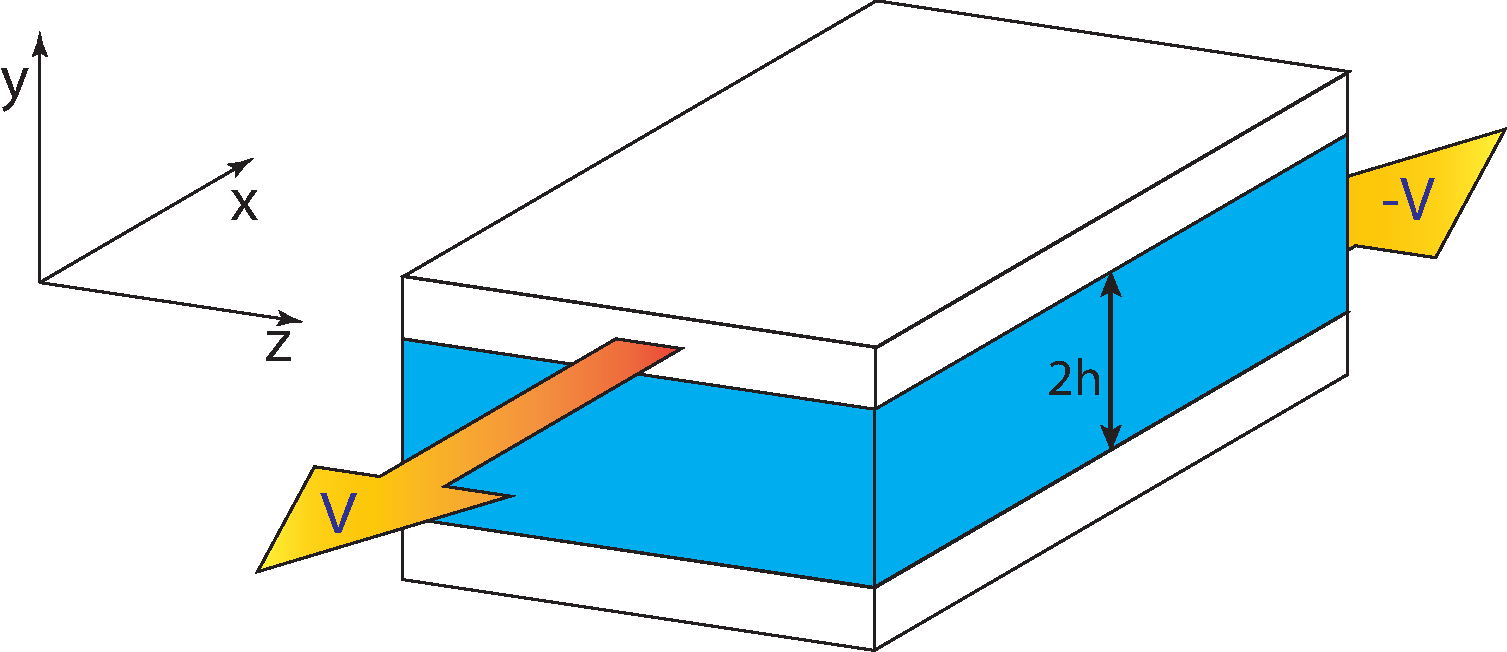
\includegraphics[scale=0.4]{Figs/planeCouetteDiagram}}
\caption{A schematic of the plane Couette geometry. The upper and lower plates (white) extend infinitely in the plane, as does the fluid (blue) filling the gap between. The upper and lower plates move with some constant velocity, and apply shear stresses on the fluid, resulting in fluid motion. While in general the plates can move in any direction, there is always a reference frame in which the plates move with equal but opposite velocity, and it is convenient to work in this reference frame. According to convention, the $x$ axis is aligned along the plate velocity, and is referred to as the {\bf streamwise} direction. The $y$-axis is aligned perpendicular to the plates and is referred to as the {\bf wall-normal} direction. The $z$-axis is normal to both axes and is referred to as the {\bf spanwise} direction.}\label{fig:planeCouette}
\end{figure}

\section{Plane Couette Flow} 

Since viscosity is a dissipative force, a viscous fluid that has no energy input will eventually have all of its kinetic energy dissipated into internal energy. Therefore, sustaining turbulence requires some form of constant energy input, which in the case of \pCf\ (\refFig{fig:planeCouette}), is provided through the shear stress of the constantly moving parallel plates. The geometry of the plane Couette system is extremely simple, with only one geometrical parameter $h$, the half-distance between the parallel plates, and one kinematic parameter $V$, the constant velocity of the upper plate\footnote{While in principle the upper and lower plate can have different velocities, there is always be a reference frame in which the upper plate has velocity $V$, and the lower plate has velocity $-V$.}, giving the Reynolds number as 
\begin{equation}
\ReN = \frac{hV}{\nu},
\end{equation}
where $\nu$ is the kinematic viscosity. When \ReN~is very small, only the laminar flow state is stable. In the case of \pCf, this corresponds to the linear velocity profile shown in \refFig{fig:planeCouetteBulk}. As \ReN~increases, experiments\rf{Daviaud1992} have demonstrated the existence of long-lived turbulent flows, even though linear stability analysis indicates that the laminar state remains stable.
\begin{figure}
\centerline{
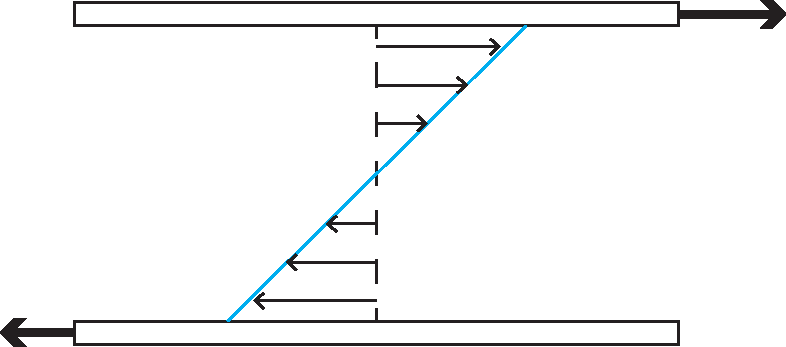
\includegraphics[scale=0.6]{Figs/planeCouetteMeanFlow}}
\caption{A cross-sectional representation of \pCf, with the linear, laminar velocity profile shown. By symmetry, the laminar profile must be the same everywhere. At the top and bottom, where the fluid meets the walls, no-slip boundary conditions require that the wall-tangent velocity equal the boundary velocity.}\label{fig:planeCouetteBulk}
\end{figure}

\section{Tackling Turbulence} 

The traditional approach for the analysis of turbulent flow is the statistical approach initially developed by Reynolds, Prandtl, von Karman, Kolmogorov and others\rf{Pope2000}. At the core of the statistical approach to turbulence is the assumption that turbulent flow states can be expressed as random perturbations around some mean flow. At high \ReN, where direct numerical simulation (DNS) of the flow is computationally infeasible, the statistical approach is invaluable, but at low-to-moderate \ReN, these models can become less accurate\rf{Pope2000}. Even ignoring the moderate \ReN\ behavior of the statistical models, the fundamental issue with the statistical approach is its discarding of the dynamical information about turbulence. Methods like Reynolds Averaged Navier-Stokes use a combination of time-averaging and modeling to eliminate small scale perturbations, while Large Eddy Simulations explicitly do not resolve small scale structures, and choose instead to model them. For this reason, it seems likely that while statistical methods are fundamental to applied computational fluid dynamics (CFD), especially in engineering practice, they cannot truly provide an answer to the turbulence problem. \\

An alternate approach was proposed by Eberhard Hopf in 1948\rf{Hopf1948}. Hopf suggested that solutions to the Navier-Stokes equations might be thought of as trajectories in an infinite dimensional state space in which each point corresponded to a possible velocity field. To better understand what this would mean, consider the mean velocity field of some infinitesimal volume of fluid, pictured in \refFig{fig:VectorSpace}. In order to describe the velocity vector, three numbers are required (each of which can take any real value), so this vector lives in a three dimensional vector space. Now any finite fluid volume will have an uncountably infinite number of points at which the velocity field has a value, so we would need an uncountably infinite set of numbers to describe any velocity field. An object that would keep track of all these numbers would form an infinite dimensional vector $\Vector{v} = \{v_{i,1},v_{i,2},v_{i,3}...\},~i \in \mathbb{R}$, so that any flow state can be represented by a particular vector in this infinite dimensional vector space, known as the {\bf state space}. 
\begin{figure}
\centerline{
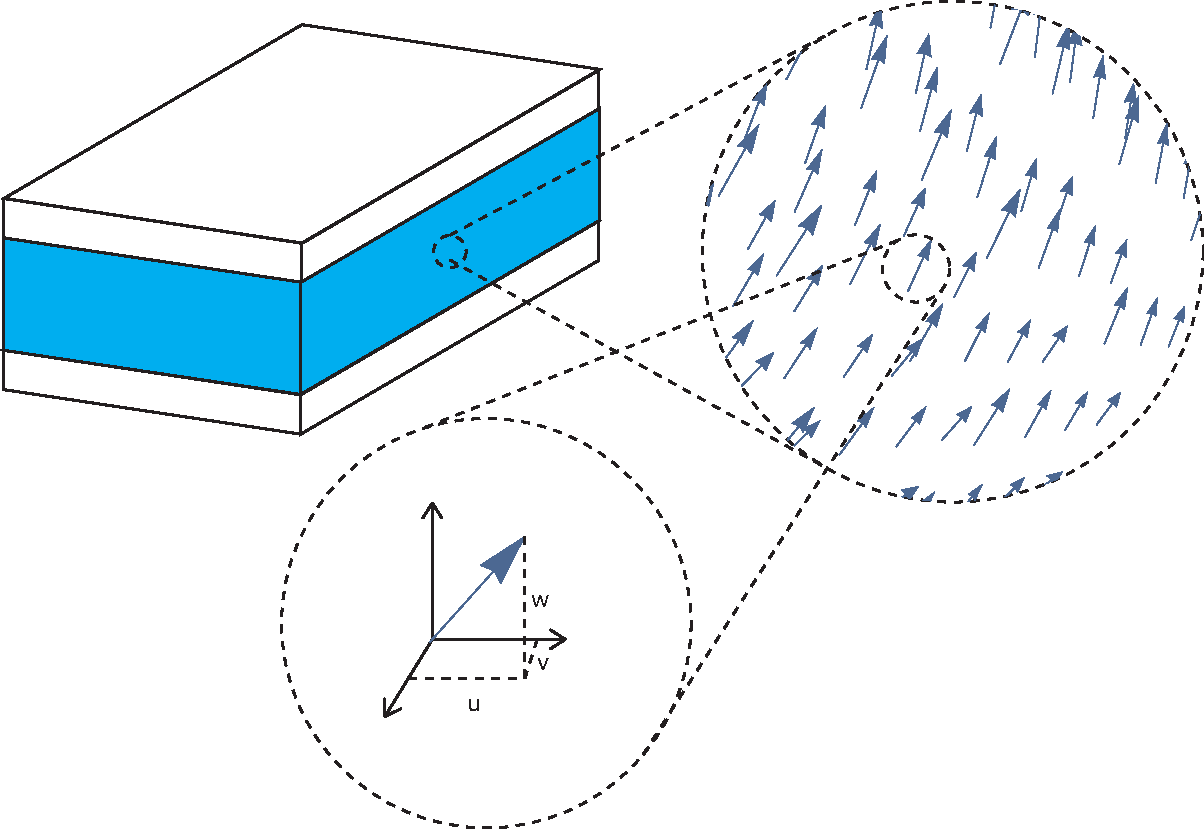
\includegraphics[scale=0.6]{Figs/VectorSpace}}
\caption{At each point in the fluid volume, the velocity field has a value that is described by three numbers, thus requiring three dimensions to track over time.}\label{fig:VectorSpace}
\end{figure}
Luckily, every point in the space does not necessarily correspond to a solution of the Navier-Stokes equation; for a given finite \ReN, for instance, the gradient of the velocity field cannot be too large. Hopf thus conjectured that physical trajectories, corresponding to solutions to the Navier-Stokes equation would lie on some finite-dimensional manifold (known as the {\bf inertial manifold}) embedded within this infinite dimensional space. The restriction of dynamics from the infinite dimensional space to a finite dimensional inertial manifold due to the variation of a control parameter has been rigorously proven under certain conditions\rf{Foias1988}. For the Navier-Stokes equation, the inertial manifold's control parameter\footnote{The control parameter of a dynamical system is a number that is time-independent, and typically dictates the behavior of the system in some way. For instance, in the dimensionless simple harmonic oscillator, $\ddot{x} + 2\zeta \dot{x} + x = 0$, the control parameter is the dimensionless number $\zeta$, whose value determines whether the system is undamped, underdamped, over damped or critically damped.} is \ReN, and physical intuition suggests that its structure should also have \ReN~dependence, since at very low \ReN, the only physical solution is the laminar state (which corresponds to the origin of the state space). As \ReN\ increases, more complex flows become physically permissible, so the inertial manifold grows from a point of dimension 0 into a more complex, higher dimensional manifold. Hopf proposed that turbulence in this view was simply a trajectory that would travel across wide distances on the inertial manifold. \\
\begin{figure}[h]
\centerline{
\includegraphics[scale=0.5	]{Figs/LorenzAttractor}}
\caption{A plot of a particular trajectory around the Lorenz attractor. The Lorenz system is an excellent example of a system in which the dynamics exist on a submanifold - in this case, the space is reduced from three dimensions to the (fractal) dimension of 2.06\rf{Grassberger2004}. }\label{fig:LorenzAttractor}
\end{figure}

Unfortunately for Hopf, the computer power necessary to pursue this line of work was not available in 1948, leading him to comment in frustration that ``“the great mathematical difficulties of these important problems are well
known and at present the way to a successful attack on them seems hopelessly
barred"\rf{Hopf1948}. It would take until 1963 and the derivation of the Lorenz attractor (\refFig{fig:LorenzAttractor}) for the first numerical state-space analysis of turbulence\rf{Lorenz1963}, albeit for a highly truncated version of Navier-Stokes, designed to investigate Rayleigh-Bernard convection\footnote{Interestingly, Lorenz truncated Navier-Stoke via a Galerkin approximation, which is what the simulation library {\tt Channelflow} which features heavily in this thesis also does, though it allows for many more Fourier modes than Lorenz did.}. There have also been a number of efforts to explore the structure of invariant manifolds in moderate turbulence Navier-Stokes, such as Proper Orthogonal Decomposition\rf{Aubry1988} and the `self-sustaining process theory'\rf{Dauchot2000}, which while fruitful, are nevertheless models of turbulent flow, and not an exact analysis of Navier-Stokes.\\

Another avenue of research emerged in 1990, when Nagata computed nontrivial {\bf equilibrium} flow states for \pCf\ by continuing the wavy vortex solution of Taylor-Couette flow\rf{Nagata1990}. This class of solutions, which were named {\bf exact coherent structures} by Waleffe\rf{Waleffe2001} are the result of calculating exact, invariant solutions of the fully resolved Navier-Stokes equations. The family of \ecs\ was expanded with the discovery of {\bf traveling wave equilibira} by Nagata in 1997, the computation of {\bf periodic orbits} by Kawahara and Kida in 2001\rf{Kawahara2001}, and the computation of {\bf relative periodic orbits}\footnote{That is, flow states that are periodic after some phase shift} by Viswanath in 2007\rf{Viswanath2007}. \refFig{fig:ECS} summarizes the four categories of \ecs.\VGC{4/8}{If I explain that in \refFig{fig:guidedTurbulence}, should I replicate that here?} The ultimate hope of this line of research is that turbulence can be viewed as chaotic trajectories on the inertial manifold that are guided by \ecs~(\refFig{fig:guidedTurbulence}). \\
\begin{figure}[ht!]
\centerline{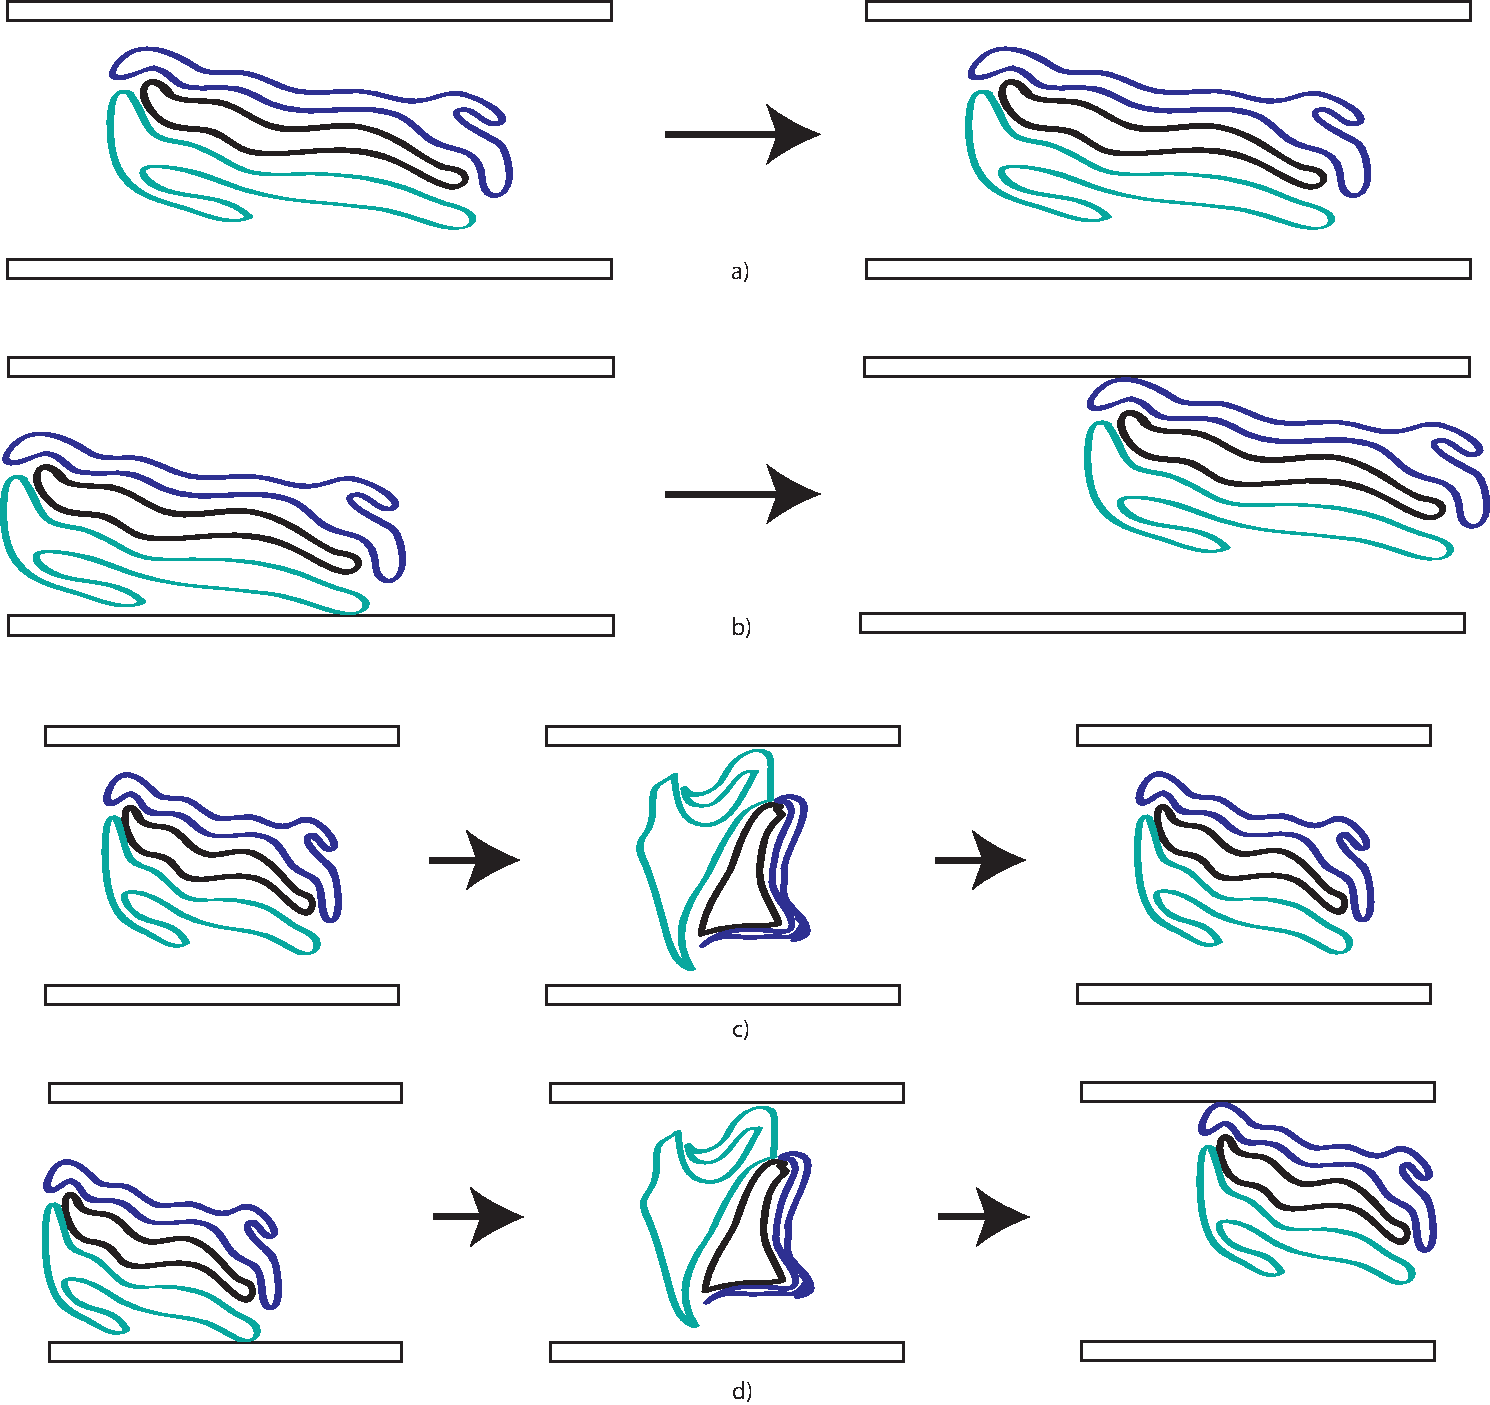
\includegraphics[scale=0.5]{Figs/ECSClassification}}
\caption{The four main categories of \ecs. In all diagrams, only a particular velocity structure of the flow state is displayed, to demonstrate the particular type of \ecs. (a) An {equilibrium} solution, where the fluid structure does not change over time. (b) A {relative equilibirum} or {travelling wave} solution, where the state does not change in its own reference frame, but is translated relative to the observer. (c) A {periodic orbit}, where the flow state changes over time, but returns to the original state after some period $T$. (d) A {relative periodic orbit}, where the flow state is periodic in its own reference frame, but is translated relative to the observer.}\label{fig:ECS}
\end{figure}


Of the work that has been done in the field, a large proportion of it has been computational, and experiments by Hof and de Lozar\rf{Hof2008}  are at present the only direct experimental verifications for the existence of \ecs~in nature. However, indirect results, such as the resemblance of Nagata's so-called `upper branch' equilibrium solution\rf{Nagata1990} to the roll-streak structure seen in DNS\rf{Gibson2008}, and the potential role of the stable manifold of the lower branch solution in separating the turbulent and laminar basins of attraction suggest that \ecs\ likely play a fundamental role in the behavior and evolution of turbulent flow states. Advances in computing power, along with the development of CFD algorithms such as Channelflow\rf{Gibson2014} have also made the computation of these structures generally feasible. In order to compute the first generation of \ecs, researchers placed substantial symmetry constraints were placed upon the dynamics. This had the benefit of greatly reduced computational cost, but has resulted in \ecs\ that are not necessarily representative of turbulence, since we expect turbulent fields to display little to no symmetry in general. As a result, while the symmetric \ecs\ 	appear to inform our understanding of turbulent transitions\rf{Halcrow2008}, they do not necessarily inform our understanding of turbulent dynamics. The focus of this thesis has been to investigate the properties of periodic orbits with broken symmetry, and how they compare to their unbroken brethren. 
 
\begin{figure}[h]
\centerline{
\includegraphics[width=\textwidth]{Figs/phaseSpaceTraj.pdf}}
\caption{A schematic of a 2D projection of a turbulent trajectory, and the coherent structures that guide it. (a) A turbulent trajectory in black appears chaotic and unpredictable in isolation. (b) When the underlying coherent structures in red are superimposed, however, the guiding of the dynamics by the \ecs\ becomes evident. Starting from the left, the trajectory is pulled in towards an equilibrium (filled circle) along a stable manifold (arrow pointing inwards), before being ejected along an unstable manifold (arrow pointing outwards). The trajectory then shadows three periodic orbits, whose stable and unstable manifolds are not trivial to visually represent, but nonetheless exist, before being attracted and ejected by the final equilibrium, after which the trajectory may continue to remain turbulent, or may relaminarize. Reproduced from D. Borrero, \emph{Subcritical Transition to Turbulence in Taylor-Couette Flow}, PhD. Dissertation, Dept. of Physics, Georgia Institute of Technology, 2014\rf{Borrero2014}.}\label{fig:guidedTurbulence}
\end{figure}
In the first chapter, I will lay out the Navier-Stokes equation and problem geometry  in further detail. In the second chapter, I will discuss the symmetries of the Navier-Stokes equations for plane Couette flow and the advantges and disadvantages afforded by considering symmetric subspaces. The third chapter will discuss in detail the spectral methods used to integrate Navier-Stokes forward in time and the Newton-Krylov-hookstep algorithm used to find coherent structures in Channelflow, along with the workflow used in this thesis. Chapter 4 presents the results of this thesis, which includes a low period orbit with broken symmetry over a large range of Reynolds numbers. Chapter 5 provides a summary of this thesis and suggests potential topics for future research. 
 
 
 
 
 